\newsection
\subsection{Law}
\label{sec:law}
\sectionauthors{Peter Henderson, Lucia Zheng, Jenny Hong, Neel Guha, Mark Krass, Julian Nyarko, Daniel E. Ho}

% \status{First draft}

\begin{figure}[!ht]
  \centering
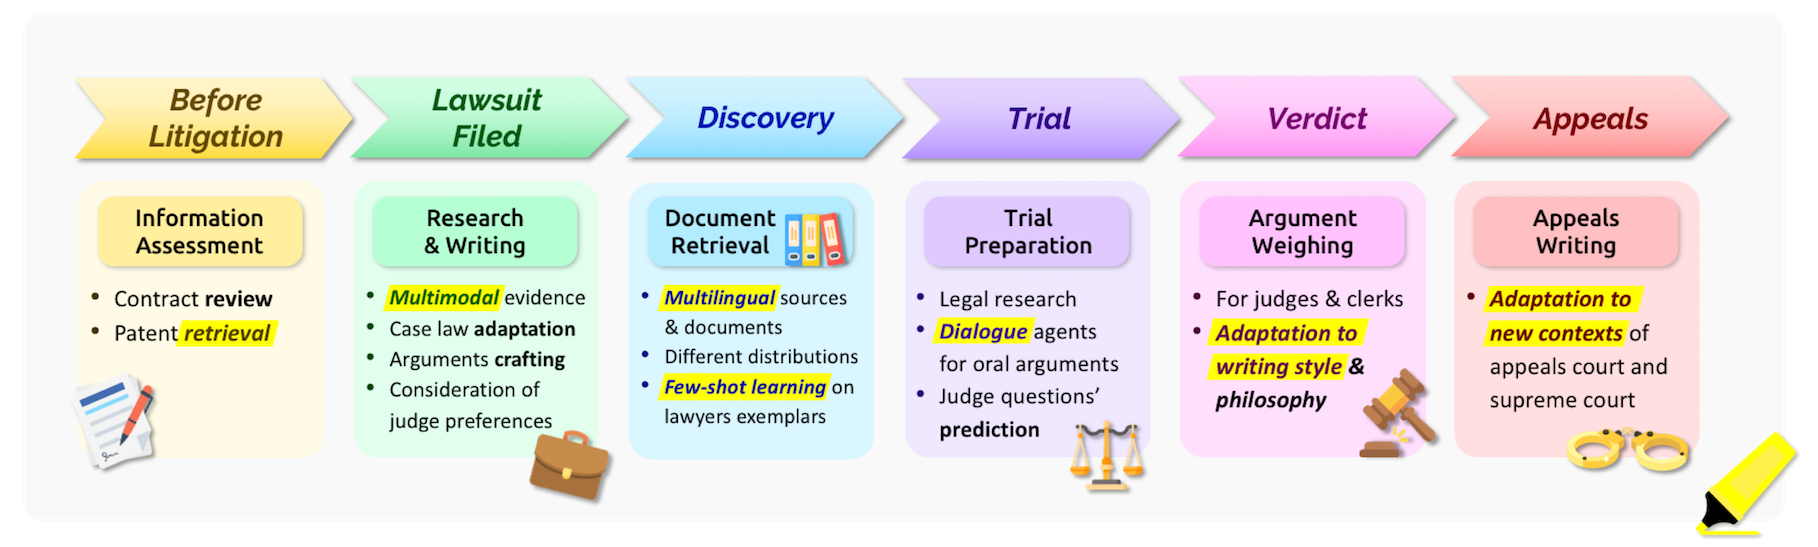
\includegraphics[width=\linewidth]{applications/law_figs/Law.png}
\caption{\label{fig:law2} An example of various steps of a civil case in the United States and where foundation models might help. At each stage different modalities might need to be processed and adaptation is needed to a new court or legal perspective.}
\end{figure}

From family court to criminal justice and from environmental policy to corporate transactions, the reach of the law is vast. In the United States,\footnote{We restrict our discussion to legal applications in the United States because of the expertise of the authors. Some discussion here may apply to legal venues globally, however.} there are over 1.3M lawyers~\citep{aba2021lawyer} and annual revenues for legal services exceed \$300B~\citep{marketline2020legalservices}.  Yet ``access to justice''  remains far out of reach for most. 
Legal services can be prohibitively expensive.
Roughly 86\% of low-income individuals with civil legal problems in the United States, for instance, report receiving inadequate or no legal help~\citep{lsc2017justice}. Even when counsel is appointed, lawyers might be strained by increasingly large caseloads. Studies have shown that public defenders, for example, are often overworked and underfunded~\citep{nrcc2009justice,nacdl2012national,aba2004gideon}. The U.S. Department of Justice reported that in 2007, 73\% of county-based public defender
offices exceeded the maximum recommended limit of cases
received per attorney and 15 of 19 reporting state public defender
programs exceeded the maximum recommended limit of felony or
misdemeanor cases per attorney~\citep{doj2010county,doj2010state}. 
%\footnote{\emph{See} \href{https://www.nbcnews.com/news/us-news/public-defenders-nationwide-say-they-re-overworked-underfunded-n828111}{https://www.nbcnews.com/news/us-news/public-defenders-nationwide-say-they-re-overworked-underfunded-n828111}.}
Even in a country with one of the highest per capita rates of attorneys, justice can appear out of reach. U.S. President Jimmy Carter once opined, ``Ninety percent of our lawyers serve ten percent of our people. We are overlawyered and underrepresented''~\citep{carter1978speech}. According to a leading voice in access to justice, technology may provide a path forward~\citep{rhode2014access}, a view echoed by many  others~\citep{cabral2012using}.
% \footnote{\emph{See, \eg } \href{https://www.americanbar.org/news/abanews/aba-news-archives/2019/05/aba-center-for-innovation-and-lsc-launch-legal-tech-donation-eff/}{https://www.americanbar.org/news/abanews/aba-news-archives/2019/05/aba-center-for-innovation-and-lsc-launch-legal-tech-donation-eff/}.}
 
What role might foundation models play in the law?\footnote{We note that for the purposes of this section we consider foundation models to be any self-supervised pretrained model that is used to quickly adapt to new contexts with little supervised learning. See also the discussion in \refsec{introduction} and \refsec{philosophy} for an expanded definition.} A major promise is that foundation models can
improve access to justice and government services by leveling procedural and financial barriers to legal services. The challenges posed by legal applications can, in turn, motivate basic research questions for foundation models. Many legal applications pose unique challenges to computational solutions. Legal language is specialized and legal outcomes often rely on the application of ambiguous and unclear standards to varied and previously unseen fact patterns. At the same time, due to its high costs, labeled training data is scarce. Depending on the specific task, these idiosyncrasies can pose insurmountable obstacles to the successful deployment of traditional models. In contrast, their flexibility and capability to learn from few examples suggest that foundation models could be uniquely positioned to address the aforementioned challenges.

Throughout this section, foundation models may take as context many modalities as evidence: audio during trial proceedings, video and images during discovery, and text in conducting legal research. Yet, the majority of legal tasks in which reliance on foundation models will be beneficial involve text-based inputs and outputs. As such, we mainly focus on text-based domains while only briefly discussing others. 
To ground the discussion, \reffig{law2} describes the stages of a civil lawsuit in the United States and where foundation models might come into play in this process. \reffig{law} shows the logic flow required to generate just part of one paragraph of a legal brief, which might serve as a concrete example of a task that foundation models might one day be used for.

\emph{An Important Consideration.} Before proceeding, we note that the ethical, legal, and fairness considerations expanded on in \refsec{ethics}, \refsec{legality}, and \refsec{fairness} are particularly important to examine before using foundation models in an applied legal or government context, as these applications often have important, real-world consequences to those affected \citep{surden2020ethics}.
Foundation models must also be thoroughly scrutinized before deployment, as discussed in \refsec{evaluation}.
For example, the legal system places particular emphasis on\dash{}and may even mandate\dash{}transparency, accountability, and explainability.
% There are also concerns that the deployment of foundation models may unduly influence decision-makers in unpredictable ways.
% Consequently, it is questionable to what extent current foundation models can be used in a production setting.
Consequently, it is questionable whether current models are positioned to solve many of the most pressing, legal problems.
Nonetheless, the need to expand and improve access to legal and government services provides a worthy goal for foundation models.  

\subsubsection{Opportunities in law}

Legal applications can range from the use of machine learning in government contexts~\citep{engstrom2020government,coglianese2020ai,re2019developing} to aiding lawyers in their provision of legal services~\citep{zheng2021does,huang2021context,ostendorff2021evaluating,vold2021using}. 
We note that prior work has also surveyed machine learning-assisted legal tasks in text-based domains~\citep{zhong2020does, chalkidis2020legal}, although it has been noted that recent legal AI research has focused on geographic regions outside of the U.S.~\citep{zheng2021does}. 
While many of the topics we discuss here may be applicable to different legal systems, due to the expertise of our team we focus primarily on the U.S. In particular, we concentrate on three broad categories of legal applications that may benefit from foundation models in the U.S. legal system: private law or civil justice (claims between private individuals, arising out of, for instance, contracts, property or torts), criminal law (\ie the prosecution of individuals for criminal behavior), and (non-criminal) public law (\eg the regulation of private behavior by government agencies).

\paragraph{Civil law.} In U.S. civil proceedings, parties must typically find and pay attorneys to be represented. As a result, many individuals, especially those with low income, struggle to secure adequate legal representation \citep{rhode2004access}. Foundation models have the potential to improve access to justice by reducing the cost, improving the quality, and extending the reach of legal services. In \reffig{law2}, we describe the process by which a civil lawsuit is filed in a U.S. court and where foundation models may play a role in aiding both attorneys and judges. 

Even before an attorney is involved in the legal process, clients may benefit from the deployment of foundation models. Recent work has used machine learning models to identify the relevant legal issues contained in a plain-language description of facts presented by a client.\footnote{\url{https://spot.suffolklitlab.org/}} Tools like these can help provide a recommendation for the type of legal action needed to address the issue at hand or to recommend a specialized attorney. A number of other similar efforts have sought to increase access to justice by providing information tailored to a client's particular needs~\citep{cabral2012using,brescia2014embracing,queudot2020improving,westermann2019using}.

Once a client speaks with an attorney, prior to civil litigation, the attorney may seek to avoid a costly trial.
At this stage, they can rely on foundation models to evaluate contracts, review terms of service, find relevant patents, and conduct other pre-litigation processes in order to ensure that their clients are at an advantage~\citep{betts2017dawn,elwany2019bert,lippi2019claudette,lee2019patentbert,hendrycks2021cuad,hegel2021law}.
Notably, recent work has both described the challenges and benefits of using foundation models for contract review~\citep{leivaditi2020benchmark,hegel2021law,hendrycks2021cuad}.
In addition to reviewing and drafting legal documents, client interactions and documents can be translated to reduce costs and barriers to the provision of legal services~\citep{cuellar_2019}.
But translation of legal documents requires precision and an understanding of highly technical language, which makes collecting training data costly.
Additionally, translating client statements or trial proceedings often requires an understanding of local dialects and language. This, too, makes it difficult to collect enough ground truth translation data to train on. As a result, traditional supervised methods rarely achieve the level of accuracy required in the legal domain~\citep{vieira2020understanding}.
Foundation models may improve performance in this area over fully supervised mechanisms by adapting quickly in these low-resource contexts. 

During litigation, foundation models can help lawyers to conduct legal research, draft legal language, or assess how judges evaluate their claims~\citep{zheng2021does,huang2021context,ostendorff2021evaluating,vold2021using, chalkidis2020legal, chalkidis2019neural}. 
This could potentially reduce the costs of and improve legal services.
For example, recent work has utilized pretrained models for the recommendation of relevant citations and holding statements when writing legal texts~\citep{zheng2021does,huang2021context,ostendorff2021evaluating}. Other work uses pretrained models for improved legal question answering to power commonly used legal search engines and help lawyers conduct legal research~\citep{vold2021using}. A wide variety of work has also examined automated contract drafting and review, a task that could similarly benefit from foundation models~\citep{hendrycks2021cuad,betts2017dawn}. Perhaps most compelling, foundation models may help assist lawyers  generate legal briefs (written arguments). The models might find novel arguments or identify problems in attorney-written portions of the brief. For example, \citet{tippett2021does} predict the outcome of a legal proceeding based on features extracted from the filed briefs. Foundation models can be leveraged to use raw language as inputs rather than extracted features. This might provide attorneys with more informative recommendations as to how their brief could be improved to ensure a favorable outcome.

After opening and reply briefs are filed, parties then begin the discovery process, which has already used simple machine learning models for the better part of a decade~\citep{grossman2010technology}. Attorneys use these systems to label whether a document should be produced to the opposing party. The documents are multi-modal in nature, often containing video, images, audio, and text.
Current systems are costly because they used supervised learning and active learning to label the documents as responsive~\citep{grossman2010technology,oard2018jointly,yang2021goldilocks}. 
Instead, few-shot or zero-shot document retrieval capabilities that might be possible with foundation models would help ease concerns about the large costs of the current process.\footnote{\href{https://www.kirkland.com/publications/article/2020/04/technology-assisted-review-framework}{https://www.kirkland.com/publications/article/2020/04/technology-assisted-review-framework}} To avoid the possibilities of gamesmanship in the discovery process, \citet{cui2018application} has proposed a zero-shot (or few-shot) adaptation process that can only be operationalized through the use of foundation models.

After discovery, once the trial begins, foundation models could help parties prepare for trial by predicting what the judge might focus on during questioning~\citep{dickinson2018computational}, adapting to the current context from judges' prior published opinions. In the courtroom, foundation models might be used to examine audio and video of courtroom proceedings to determine if outcomes were biased against the defendant because of their race or dialect.\footnote{For example, speaking African-American Vernacular English dialects in the courtroom has been shown as a potential source of bias during trial. \url{https://www.nytimes.com/2019/01/25/us/black-dialect-courtrooms.html}}

Once the trial concludes, foundation models could help judges and law clerks to properly evaluate legal claims from both parties using similar technologies, or the use of contextual embeddings from foundation models might assist in statutory interpretation~\citep{nyarko2020statistical,choi2020empirical}. Recent work (without reliance on foundation models or NLP) has examined whether an appeals decision can be predicted from a set of extracted features, like citation counts and the appearance of key words~\citep{katz2017general,boniol2020performance}. It is possible that such models could be improved using foundation models and applied to help judges draft decisions by flagging obvious mistakes in their opinion, as has been discussed in the context of adjudicative agencies~\citep{engstrom2020government,ray2014government}. They can also be used to identify racial biases in legal opinions and help judges revise their opinions accordingly~\citep{rice2019racial}.

\paragraph{Criminal law.} One particularly contentious area has been the use of risk scores in government settings, particularly in criminal law. Some may want to use language-based foundation models to aid in making charging decisions or parole decisions based on a given text-based narrative of the events. Careful consideration must be taken before using foundation models for risk scoring due to the potential for biases, especially when language data is included~\citep{bender2021,berk2021justice,laufer2020feedback}. But foundation models may play a role in many other dimensions of criminal justice. 
The same tools as in civil litigation, above, can also be used by prosecutors and defense attorneys. This can help appointed attorneys perform their job more efficiently and reduce unnecessary overhead. As a result, they may be able to balance already heavy caseloads more effectively. For example, public defenders are often viewed as being overworked and underfunded, which would lead to avoidable procedural errors.\footnote{See, for example, in \textit{People v. Superior Court (Vasquez)}, 27 Cal.App.5th 36 (2018) a defendant did not receive a trial for 17 years because the public defender's office had severe budget cuts and understaffing. The court ruled that the systemic breakdown in the public defender's office constituted a due process violation and the defendant's case was dismissed.} Foundation models can help reduce \textit{some} of these resource constraints by identifying errors and automating simple tasks. However, they are not a solution on their own.

In other areas, foundation models can act as an oversight mechanism to reduce structural inequities. pretrained models have been used for processing parole hearing transcripts to find instances of anomalous outcomes~\citep{bell2021recon}. Recent work has also removed linguistic cues for a suspect's race in police reports to promote race-blind charging decisions and avoid racially biased prosecutions~\citep{chohlas2020blind}. Other work has helped identify disrespectful police communications~\citep{voigt2017language}. 
In these contexts, it is very costly to label data since annotators must be given access to sensitive data and appropriate background checks are often required. To reduce these costs, foundation models can be used to pretrain and adapt quickly to downstream tasks where labels are scarce. 

\paragraph{Public law.} Government agencies regulate vast parts of society, and foundation models have wide potential applicability across public law. This includes: analyzing public comments in the notice-and-comment process, assisting  patent examination, retrieving relevant documents in response to Freedom of Information Act requests, aiding in mass adjudication, among many others. 
Recent work has surveyed these government applications in a variety of contexts and we refer the reader to the relevant sources for in-depth discussion~\citep{engstrom2020government,coglianese2020ai}. 
In many of these applications, foundation models can improve the quality, efficiency, utility, and accessibility of government services: labels are scarce, resources are constrained, and contexts are constantly shifting. As such, the adaptability and flexibility of foundation models are often required to improve efficiency and performance.
To give an illustrative example of just one such application, existing work has leveraged NLP for facilitative moderation in public comment forums. In this use case, predictive models help lay-users improve arguments and identify misstatements in their comments. Such a system has already been deployed in the U.S. Department of Transportation rulemaking process~\citep{park2012facilitative}, although it can likely be improved through the linguistic reasoning capabilities of foundation models.
But government agencies must comply with constitutional, statutory, and administrative obligations (see \refsec{legality}), so additional care is needed in these settings. 

\subsubsection{How can foundation models uniquely help?}

The above examples of legal applications are unique in several ways. First, the cost of annotating data is very high. Often, the expertise to create high-quality labels can only be found in attorneys, who may charge hundreds of dollars per hour. %\footnote{It is possible to automate labeling~\citep{zheng2021does} for some tasks. Some efforts have been made to create large benchmarks on a specific subdomain through crowdsourced expert annotation~\citep{hendrycks2021cuad}. Such benchmarks can be helpful where data can be released and the task is sufficiently broad.} <- weaved this in to a later subsection on Access to Clean In-Domain Data
Even after labels are obtained, certain data may be sensitive and cannot be pooled together to training a large language model.
% This means that models must both take into account complex linguistic patterns often associated with nuanced legal decision-making and do so in a few-shot manner.
% In fact, the repeated theme in the above cases is that in most legal domains, resources are constrained and labels are costly.
Given recent progress in few-shot learning~\citep{brown2020gpt3}, foundation models are among the most promising paths for learning models with limited annotations.

Second, legal decision-making requires context at various scales: knowledge of all historical decisions and standards, knowledge of the case law that remains relevant in the present, and knowledge of the nuances of the individual case at hand. Foundation models are uniquely poised to have the potential to learn shared representations of historical and legal contexts, as well as have the linguistic power and precision for modeling an individual case. 

\subsubsection{What are foundation models lacking that requires more research?}

\begin{figure}[t]
  \centering
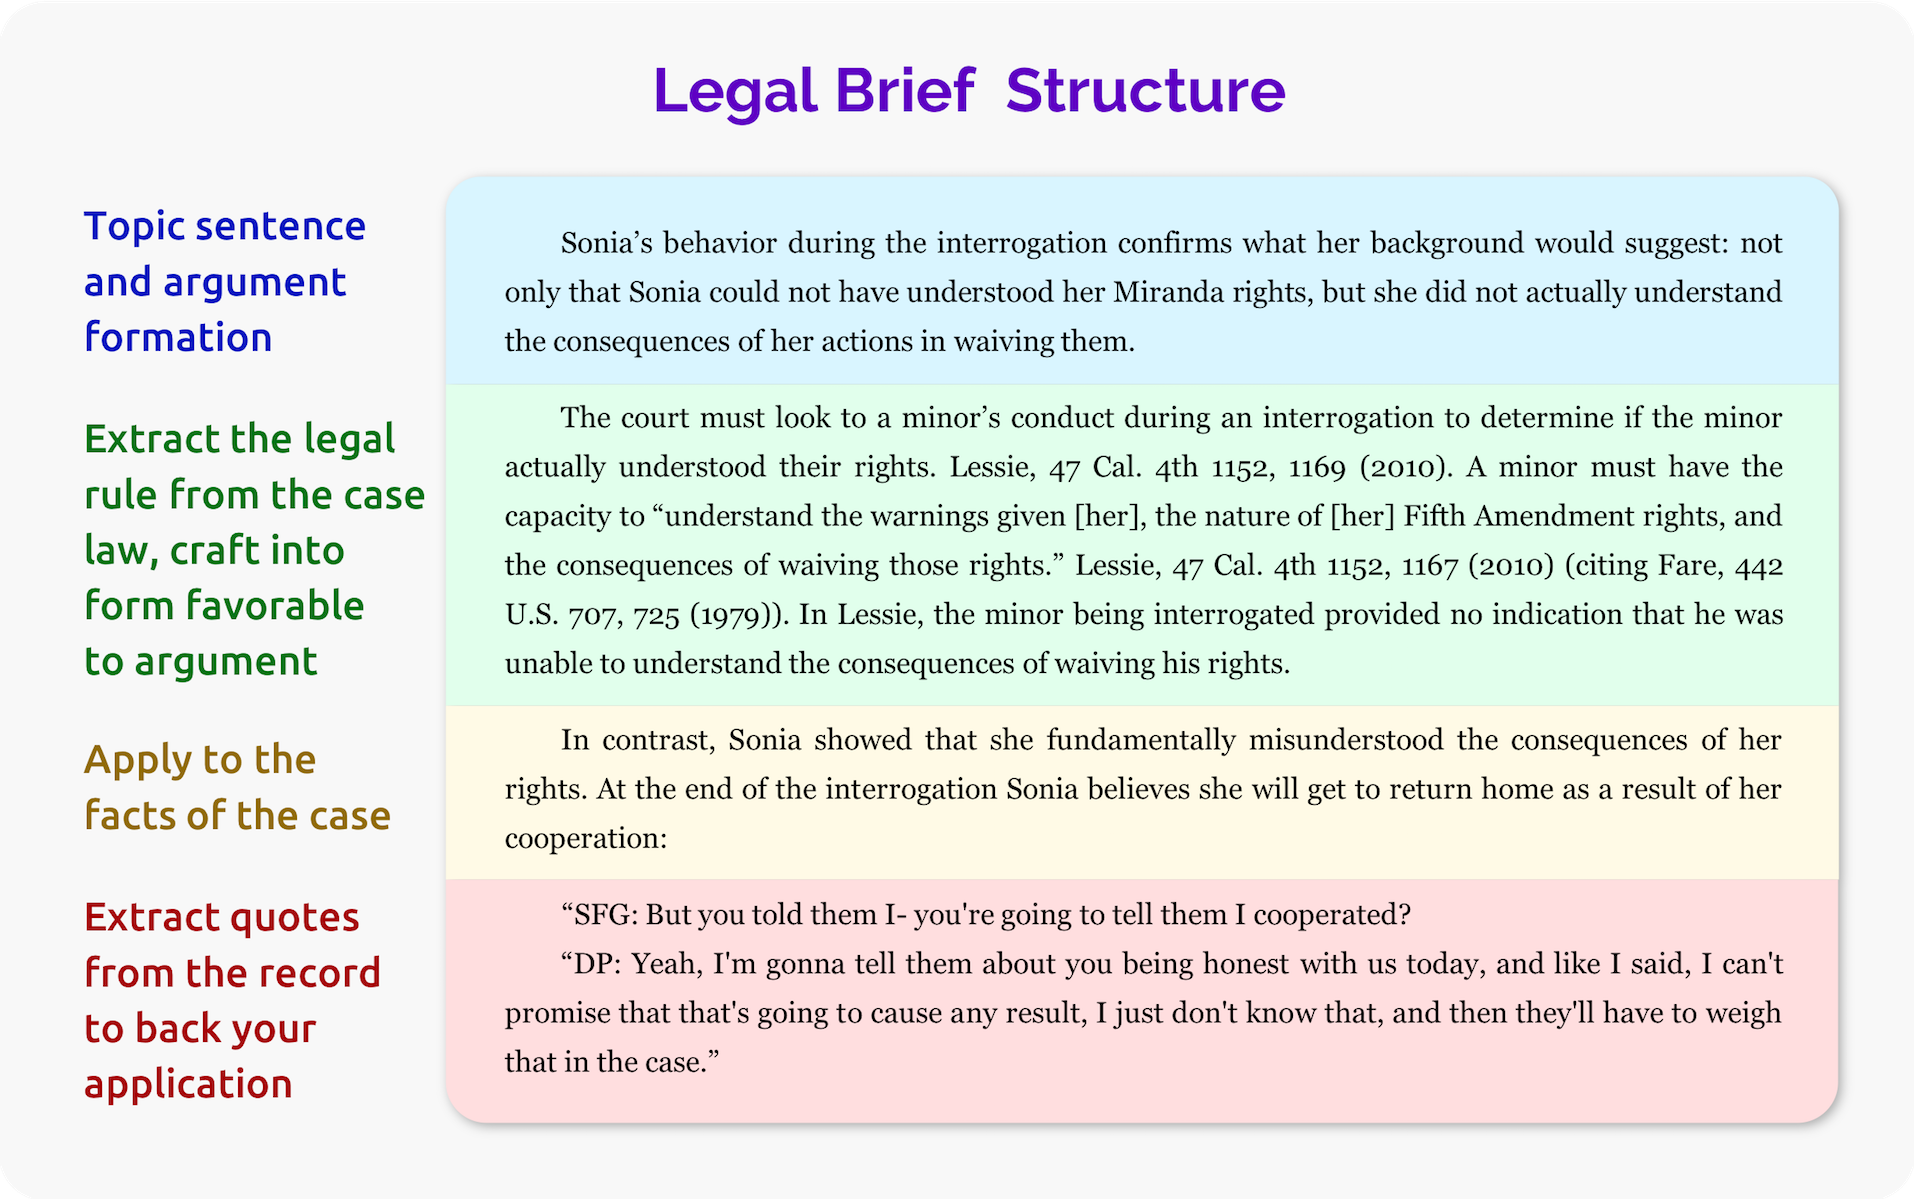
\includegraphics[width=\linewidth]{applications/law_figs/Law_brief.png}
\caption{\label{fig:law} An extract from a fictional brief written by one of the authors of this work. The prototypical form that law students are instructed to write a brief involves: (1) introducing the argument; (2) stating the legal rule in a persuasive manner; (3) applying the legal rule to the facts of the case; (4) persuasively concluding the argument. This often involves information retrieval and paraphrasing from both prior cases and the facts of the current case.}
\end{figure}

% More improvement on this front is likely needed to adapt to complex legal settings.
% \emph{Can foundation models write a legal brief in their current state?}
To illustrate the deficiencies current foundation models need to overcome in order to be realistically deployed, we consider as an example the automatic creation of a legal brief to submit to a court.

A brief lays out the arguments to a judge before a hearing. Once a party has filed an opening brief, the opposing party files a response. The judge then evaluates the briefs and asks questions of both parties at a hearing before making a decision. \reffig{law} visualizes the structure of such a legal brief with some of its characteristic features.

An automated brief generation mechanism might take as context relevant documents and facts of a case (as specified by an attorney) as well as a rough sketch of the desired outcome. It would then generate a legal brief with complex legal arguments to submit to the court. 
\medskip

\textit{Long Documents and Narratives.} To achieve this goal, the model must be able to read long contexts and produce long narratives.
Legal documents tend to be far longer than documents in any other context. The average U.S. Supreme Court opinion contains around 4,700 words,\footnote{\href{https://www.americanbar.org/groups/public\_education/publications/teaching-legal-docs/how-to-read-a-u-s--supreme-court-opinion/}{https://www.americanbar.org/groups/public\_education/publications/teaching-legal-docs/how-to-read-a-u-s--supreme-court-opinion/}} a brief on the merits to the Supreme Court can have as many as 15,000 words,\footnote{\href{https://www.supremecourt.gov/casehand/courtspecchart02162010.aspx}{https://www.supremecourt.gov/casehand/courtspecchart02162010.aspx}}
a law review article often contains 20,000 to 30,000 words,\footnote{\href{https://www.stanfordlawreview.org/submissions/article-submissions/}{https://www.stanfordlawreview.org/submissions/article-submissions/}}
parole transcripts can be hundreds of pages long~\citep{bell2021recon}, and trial records can be even longer.
Current foundation models have struggled with such long contexts and outputs (see \refsec{modeling} for more discussion).
\medskip
% , though there have been rapid improvements.

\textit{Retrieval, Concept Drift, Argument Formation, and Logical Reasoning.} In addition to reading case-specific documents, the foundation model must retrieve the relevant case law and understand which case law is still valid and which has been overruled, taking into account potential concept drift since it was trained. More work in editing grounded information in foundation models will be required as case law evolves~\citep{de2021editing}. Using retrieved legal standards, the foundation model must then understand how to weave them into a persuasive argument. Emerging research has studied ways of using foundation models to measure, detect, and generate persuasive texts~\citep{duerr2021persuasive, li-etal-2020-exploring,longpre-etal-2019-persuasion}, which may provide stepping stones towards this goal.

But legal briefing also requires the ability to identify a relevant legal rule and determine how it applies to a new situation.
For example, \citet{holzenberger2020dataset} provide a dataset and methodology for evaluating this ability in current models based on the tax code. 
Given a set of tax code rules and a description of someone's situation, the model must determine how the rules apply to the individual in order to determine what their tax liability is.\footnote{For example, a rule might look like, ``In the case of an individual who is not married and is
not a surviving spouse, paragraphs (1) and (2) shall be
applied by substituting `\$750' for `\$600'.'' US Internal Revenue Code (IRC) \S 63(f )(3).}
\citet{holzenberger2020dataset} found that domain experts can express the relevant tax law as a prolog solver to determine an individual's tax liability with perfect accuracy. However, they found that simply using a BERT model, even when pretrained on in-domain legal text, was not sufficient to allow the model to deduce and apply the relevant rules, a process also referred to as ``legal reasoning.'' 

These challenges can further be illustrated through a real exchange with GPT-3, demonstrating that current models are unable to perform even comparatively simple tasks involving legal reasoning.

\begin{tcolorbox}[breakable, enhanced]
\begin{center}
\textbf{Legal Reasoning with GPT-3.} 
\end{center}

``Liquidated damages'' are a form of monetary compensation for a breach of contract that the parties specify in their agreement. In general, courts in the U.S. will not enforce liquidated damages provisions if the amount stipulated in the contract is so high that it acts as a form of punishment, rather than to be merely compensatory.

First, we see if the model encoded the correct rule about the enforcement of liquidated damages provisions.

\begin{dialogue}
\speak{Q} Are liquidated damages clauses enforceable?
\speak{A} Liquidated damages clauses are generally enforceable unless the sum stipulated is exorbitant or unconscionable.
\end{dialogue}


The rule appears correct. But then we apply the rule to a set of facts. Here, the model needs to infer that one million in damages is exorbitant for a Toyota Corolla and thus, the liquidated damages provision should not be enforced.

\begin{dialogue}
\speak{Q} X and Y contract over the sale of a Toyota Corolla. Their contract specifies that X has to pay Y one million dollars in damages if X does not deliver the car on time. X does not deliver the car on time. Is Y entitled to damages? If so, in what amount?
\speak{A} Yes, Y is entitled to \$1,000,000 in damages. Damages are meant to compensate the injured party for the loss suffered due to the breach. Y has suffered a loss of \$1,000,000 because X has not delivered the car on time.
\end{dialogue}

The model is unable to infer that \$1M for a Toyota Corolla is exorbitant. Even if the model is provided with both the abstract rule and its precise translation to the context in the prompt\dash{}and the application should thus be trivial\dash{}GPT-3 is still unable to conduct the logical reasoning required.

\begin{dialogue}
\speak{Q} X and Y contract over the sale of a Toyota Corolla. Their contract specifies that X has to pay Y the exorbitant amount of one million dollars in damages if X does not deliver the car on time. X does not deliver the car on time. The law requires that liquidated damages clauses are enforced unless the sum stipulated is exorbitant or unconscionable. Is Y entitled to damages? If so, in what amount?
\speak{A} Yes, Y is entitled to the liquidated damages. The amount in this case is not exorbitant since the price was set by the parties themselves.
\end{dialogue}
\end{tcolorbox}

\medskip

\textit{Precision.} The foundation model also cannot create fake facts in the process, a problem that has come up in current models~\citep{gretz2020workweek,zellers2019neuralfakenews}. Specificity and truthfulness are of heightened important in legal contexts, where imprecise statements can have drastic, unanticipated consequences, and false statements can lead to sanctions against attorneys.

\medskip

\emph{Few-shot Learning.} Some challenges facing foundation models beyond those described in the above example include few-shot learning, which is still in its infancy~\citep{perez2021true}. Research on few-shot learning techniques and increasing access to legal corpora can work in tandem. Because foundation models need to be precise, not only in factual truth, as discussed above, but also in technical legal language, it remains unclear to what extent information obtained from one corpus can be utilized in another corpus of a different domain. Few-shot learning thus remains important.
\medskip

\emph{Adaptation.} Some gains have been observed from domain-adaptive pretraining on unlabeled legal corpora. These gains appear to be most pronounced when the pretraining corpus is highly relevant to the downstream task and labeled training data is limited (a setting which is common in the law) \citep{zheng2021does}. It has not yet been comprehensively studied whether this extends to a diverse set of legal tasks, but leveraging unlabeled domain-specific corpora for self-supervised training of foundation models may provide complementary improvements to few-shot methods.
\medskip

\emph{Access to Clean In-Domain Data.} Some recent efforts have sought to create large labeled datasets for more challenging legal benchmark tasks through automation~\citep{zheng2021does} or manual annotation by volunteer legal experts~\citep{hendrycks2021cuad}. These efforts have demonstrated that larger language models that are pretrained on more data achieve performance gains on certain challenging tasks, compared to more limited gains observed in other settings~\citep{chalkidis2020legal, elwany2019bert, zhong2020does}. This work suggests that larger legal benchmark datasets may be necessary to observe further gains from applying transfer learning techniques to foundation models. However, creating benchmark datasets for tasks that are legally meaningful and difficult from an NLP perspective can itself be challenging, as human expert annotation can be costly and automated methods that utilize conventional tokenization and sentence segmentation techniques can fail to account for unique aspects of legal text, such as the structure of legal citations~\citep{bommarito2018lexnlp,savelka2017sentence}. As a consequence of these challenges, many existing legal domain-specific labeled datasets are small, not publicly available, or reflect simpler tasks that have been solved by methods often pre-dating the development of foundation models.\footnote{For law firms and legal technology companies, tasks for which high performance can already be achieved, and can therefore be more immediately productized, may be considered more worthwhile to invest costly manual labeling efforts towards.}

Much available legal data may also be unrepresentative. Since only a fraction of cases end up in legal opinions, it is unclear whether the disputes in publicly available data are representative of the typical disputes presented to a model in practice~\citep{priest1984selection}.
Costly training data for more representative scenarios may be concentrated in the biggest law firms.
These law firms may have the ability to retain and accumulate data across many cases and clients. One concern then is that foundation models could concentrate power even more among the few actors that have the resources to train models on in-domain data\dash{}unless the models can generalize sufficiently well.
\medskip

\emph{Reliability.} Finally, we again note that even if foundation models could successfully perform all tasks in the legal domain, deployment remains a major challenge: a failure of a foundation model in the law will have real, damaging consequences to both clients and attorneys (see also discussion on fairness, legality, and ethics in \refsec{fairness}, \refsec{legality}, and \refsec{ethics}).
For this reason machine translation software has already been deemed unreliable for use as evidence in some courts,\footnote{See discussion by \citet{vieira2020understanding}.} although it continues to be relied upon in others.\footnote{For example, in \textit{Vasquez v. United States}, No. 3: 16-cv-2623-D-BN (Dist. Court, ND Texas 2019), counsel relied on Google Translate to prove that the previous (native speaker) attorney has mistranslated a plea deal.}

Given all of these complexities, legal briefing and reasoning is likely beyond the capabilities of current models, but appears to be within the future realm of possibilities. As such, these serve as a potential lode star for the ongoing development of foundation models.




